\documentclass[10pt,a4paper]{article}
\usepackage[utf8]{inputenc}
\usepackage[italian]{babel}
\usepackage{amsmath}
\usepackage{amsfonts}
\usepackage{amssymb}
\usepackage{graphicx}
\usepackage{gensymb}
\usepackage[left=2cm,right=2cm,top=2cm,bottom=2cm]{geometry}
\newcommand{\rem}[1]{[\emph{#1}]}

\author{Gruppo BN \\ Federico Belliardo, Marco Costa, Lisa Bedini}
\title{Lock in}
\begin{document}

\maketitle
\section{Scopo dell'esperienza}
Questa esperienza è finalizzata alla misura della costante di assorbimento del Mylar. Nella prima parte ci si propone di montare i circuiti e caratterizzarne il singolo funzionamento, successivamente procederemo a collegarli fra loro per eseguire la misura mediante lock-in.

%Si misurerà potenziale in funzione del numero di lastrine di Mylar\footnote{Resina termoplastica di indice di rifrazione pari a 1.5750 (utile?)} (e quindi ricavare il coefficiente di assorbimento di tale materiale) interposte fra la sorgente luminosa (LED) e il fotodiodo (fototransistor?). Infine verificheremo che il sistema non è sensibile alla luce ambientale\footnote{Una delle tante sorgenti di rumore.}%

\section{Materiale occorrente}
\begin{itemize}
\item TL082 (JFET input dual Op-Amp);
\item 4 TL081 (JFET input Op-Amp);
\item SN7400 (4 porte NAND);
\item DG441 (4 interruttori analogici CMOS);
\item 2N1711/BC182 (transistor NPN);
\item LED rosso;
\item fotodiodo;
\end{itemize}


Tutte le resistenze, i condensatori e la tensione di alimentazione sono stati misurati con il multimetro digitale, quindi l'errore è stato propagato secondo le specifiche nel manuale ($0.8\% + 3$digit per le resistenze e $0.5\% + 1$digit per i voltaggi). I tempi e le restanti tensioni sono state misurate con i cursori dell'oscilloscopio: l'errore sui tempi è dato dalla risoluzione dei cursori stessi mentre quello sulle tensioni è stato propagato considerando sia l'errore sul posizionamento dei cursori sia l'errore sistematico del $3\%$.

\section{Schema a blocchi}
Il circuito Lock-in è usato per effettuare misure di segnali deboli in un ambiente molto rumoroso. Nel nostro caso il segnale è la luce emessa dal LED. Tale segnale non è continuo ma modulato da un' onda sinusoidale prodotta dal generatore di funzioni. Abbiamo scelto una frequenza pari a $1\,\mbox{kHz}$ per eliminare il rumore \emph{1/f} dovuto alla presenza di dispositivi attivi\footnote{Può essere prodotto dalle discontinuità intrinseche dei materiali costruttivi.}. In figura \ref{fig:schemablocchi} si nota come questo circuito complesso sia costituito da sottocircuiti (che saranno analizzati e spiegati successivamente); in particolare nella parte superiore dello schema si trovano i circuiti che servono a sfruttare sia la parte positiva che negativa del segnale per la misura e nella parte inferiore si trovano i circuiti di amplificazione del segnale da misurare.

\begin{figure}[!htb]
  \centering
  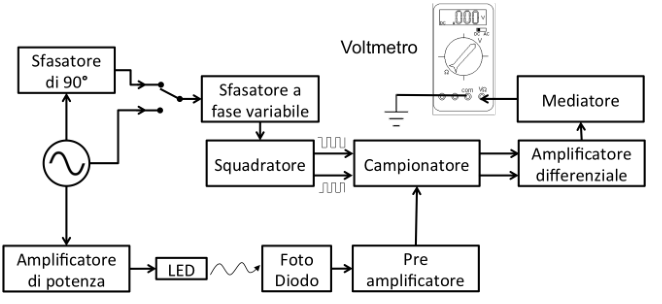
\includegraphics[scale=0.75]{schemablocchi.png}
\caption{Schema a blocchi del circuito Lock-in.\label{fig:schemablocchi}}
\end{figure}


\section{Implementazione schema a blocchi}

\subparagraph{Amplificatore di potenza e preamplificatore}
Abbiamo montato il circuito in figura \ref{fig:ampli-preampli} misurando tramite multimetro digitale: $R_1=10k$, $R_2=1.5k$, $R_3=82k$, $R_4=56k$, $R_5=18k$, $R_6=120k$, $R_7=3.9k$, $R_9=1.2M$, $C_1=100n$ e $C_2=100n$.\\
%vpp 5.92   freq 1.035 kHz
%rumore 
%
%ampiezza ch2 
Il circuito consiste in un amplificatore di potenza realizzato con un transistor npn che permette di pilotare l'accessione del Led con l'onda del generatore di funzioni, che controlla la corrente in base.
Il transistor è dotato di circuito di polarizzazione quindi come anticipato prima l'effetto del segnale alternato è di modulare la corrente di collettore e quindi l'intensità luminosa.
Nella seconda parte (elettricamente separata dalla prima) troviamo un  circuito di lettura del fotodiodo, che grazie all'opAmp presenta un alta impedenza di ingresso e bassa impedenza di uscita e permette quindi di osservare la risposta del diodo senza alterarla.
Il segnale del fotodiodo viene poi derivato (per ottenere un segnale a media nulla) e mandato in un comune amplificatore non invertente dal guadagno di circa $A = 30$.\\

\subparagraph{Misura della costante di assorbimento senza Lock-in}
Per limitare l'influenza della luce ambientale tutte le seguenti misure sono state eseguite coprendo l'apparato con %TODO %che cosa?%.
Si è inviato all'ingresso (S1) un segnale sinusoidale di frequenza pari a $1 kHz$ e ampiezza picco-picco $V_{pp}= 6 \pm \,\mbox{V}$. All'uscita (S6) si ottiene la forma d'onda sinusoidale in figura \ref{fig:S6} che ha ampiezza TOT. Abbiamo ripetuto la misura della tensione in uscita in funzione del numero $n$ di lastrine di Mylar poste fra LED e fotodiodo, i dati sono rappresentati in tabella \ref{tab:ampli-preampli}. Sapendo che l'andamento teorico della tensione è $V_{out}=V_0exp(-n/n_0)$ si è fatto il grafico e eseguito il fit, ottenendo $n_0= V_0= \chi^2=$. Conoscendo lo spessore costante delle lastrine ($150\mu \mbox{m}$) si osserva che il numero $n$ è direttamente proporzionale alla lunghezza percorsa dalla luce nel Mylar. Sostituendo otteniamo direttamente a esponente della legge la lunghezza caratteristica di assorbimento: $x_0= TOT$.

\begin{figure}[!htb]
  \centering
  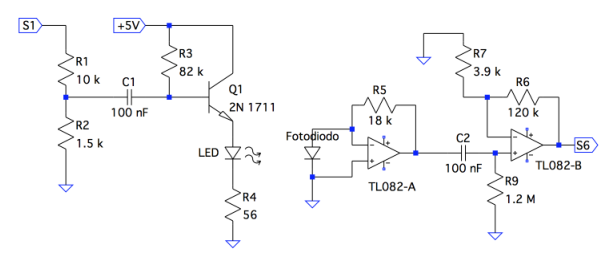
\includegraphics[scale=0.75]{ampli-preampli.png}
\caption{Schema a blocchi del circuito Lock-in.\label{fig:ampli-preampli}}
\end{figure}

IMMAGINI OSCILLOSCOPIO USCITA E RUMORE PER STIMA
TABELLA DATI
GRAFICO E FIT VvsNUMERO LASTRINE
SENSIBILE A LUCE AMBIENTALE? sì infatti abbiamo fatto caso a prendere le misure con meno luce ambientale possibile
%Dire eventualemnte se si osserva rumore alla frequenza delle lampade, che è 50 Hz$
%v picco picco quindi errore grande
\begin{table}
\centering
\begin{tabular}{c|c|c}
\hline
n	&	$V_{out}\,\mbox{[V]}$	&	$\Delta V\,\mbox{[V]}$\\
\hline
0 &  3.16  &  0.03\\
\hline
1  & 2.96  &  0.03\\
\hline
2 &  2.48  &  0.02\\
\hline
3  & 2.12   & 0.02\\
\hline
4   &1.92   & 0.02\\
\hline
5   &1.62    &0.02\\
\hline
6   &1.12   & 0.01\\
\hline
7   &0.8    & 0.01\\
\hline
\caption{Presa dati della tensione in S6.\label{tab:abs1}}
\end{tabular}
\end{table}
n	v
0	3.16
1	2.96
2	2.48
3	2.12
4	1.92
5	1.62
6	1.12
7	0.800


\subparagraph{Sfasatore di 90\degree e sfasatore variabile}
I circuiti relativi sono quelli in figura \ref{fig:sfasatori}. L'ingresso S1 è ancora riferito all'uscita del generatore di funzioni. Abbiamo regolato il trimmer P1 in modo da ottenere in S2 la stessa forma d'onda dell'ingresso sfasata di 90\degree (figura \ref{osc:sfasatore90}). In S3 l'uscita sarà un'onda quadra e abbiamo regolato il trimmer P3 in modo che il \emph{duty cycle} fosse pari al 50\% (ciò è stato verificato con l'opportuna funzione dell'oscilloscopio). Se si agisce sul deviatore si bypassa lo sfasatore quindi all'ingresso dello sfasatore variabile l'onda sarà la stesa in ingresso a S1.\\
L'analisi dello sfasatore mostra che esso ha una funzione di trasferimento nel dominio di Laplace: $G(s) = -\frac{1-s(R_{16} +P_1) C_{4}}{1+s(R_{16} + P_1)C_{4}}$ dunque si tratta di una fase che può essere scelta calibrando il trimmer $P_1$. Esiste un solo valore della resistenza di trimmer per cui a $1$kHz si ha uno sfasamento positivo di $\frac{\pi}{2}$\\
L'analisi del circuito che regola il duty cycle si presenta simile, l'uscita S3 risulta in questo caso essere:
\begin{equation}
v_{out}(s) = \left( \frac{s C_3 (R_{13} + P_2)}{1 + s C_3 (R_{13} + P_2)} \frac{R_{12}}{R_8+P_3} -\frac{1-s(R_{13} +P_2) C_{3}}{1+s(R_{13} + P_2)C_{3}} \right) V_{in}-\frac{R_{12} V_{EE}}{R_8+P_3}
\, \, \, \, \, \, ; V_{EE} = -5V.
\end{equation}
%C'è anche una attenuazione da passa alto
Come si vede l'output presenta un offset costante positivo $-\frac{R_{12} V_{EE}}{R_8+P_3}$ il cui valore massimo risulta essere circa $0.61$V. L'aumento della resistenza $P_3$ si vede che causa una diminuzione anche dell'ampiezza del segnale proporzionale a $V_in$. 

\begin{figure}[!htb]
  \centering
  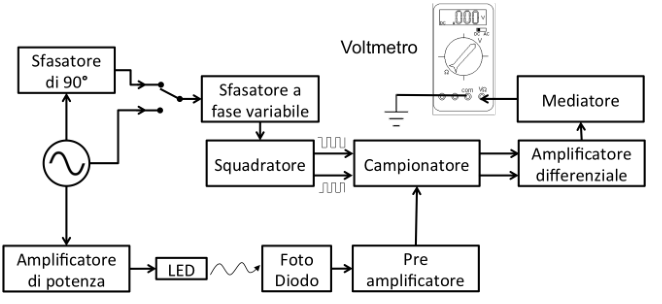
\includegraphics[scale=0.75]{schemablocchi.png}
\caption{Schema a blocchi del circuito Lock-in.\label{fig:schemablocchi}}
\end{figure}

Il circuito applica anche uno sfasamento rispetto al segnale originario regolabile con $P_2$. L'uscita viene mandata alla base di un transistor la cui polarizzazione è tale da potersi muovere sulla retta di carico solamente (in pratica) tra la zona di saturazione e quella di interdizione. Il segnale in arrivo sulla base è molto vicino alla tensione di polarizzazione diretta della giunzione BE, dunque la variazione dell'ampiezza della componente oscillante che arriva in base è direttamente legata alla frazione di tempo per cui questo segnale è sufficientemente alto da polarizzare in diretta la giunzione BE mandando quindi il transistor in saturazione. Variare $P_2$ varia in effetti della stesso fattore sia la componente continua che quella oscillante della tensione sulla base, quindi di fatto agisce come un coefficiente di dilatazione che permette al segnale di attraversare la barriera di potenziale oltre a cui si ha saturazione per una frazione controllabile del periodo.
Il transistor alternativamente in saturazione e interdizione produce su S3 un'onda quadra (sfasata di $\pi$ rispetto al segnale in base ma è irrilevante).\\


\begin{figure}[!htb]
  \centering
  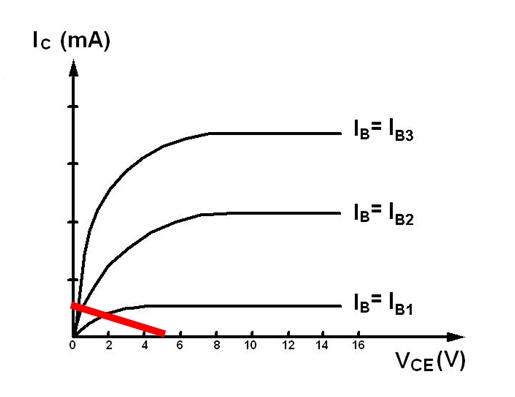
\includegraphics[scale=0.75]{transistor.jpg}
\caption{Retta di carico del transistor.\label{fig:transistor}}
\end{figure}

Come si vede in figura \ref{fig:transistor} la retta do carico del transistor (in rosso) è molto bassa e non permette mai di entrare veramente in regime attivo. Variare la tensione sulla base commuta quindi il transistor tra gli stati di interdizione e di saturazione.\\

%TODO : Verdficare questa ipotesi e prendere una immagine del segnale il base da schiaffare. Sull'immagin della tenzione in base disegnare la tenzione a cui il transistor viene mandato insaturazione.
%Lo sfasamento dello sfasatore 1 è pi-2arctg(omega/(R16+p1)*C4)
%a basse frequenze lo sfasamento è automaticamente 90gradi
%556/968
%500/980 duty cycle
%escursione di fase con trimmer fase: 4/5pi

LIMITI TRIMMER P2 PER REGOLARE SFASAMENTO - Misurare
IMMAGINI CON E SENZA DEVIATORE 
IMMAGINI ONDE ALLE USCITE

\begin{figure}[!htb]
  \centering
  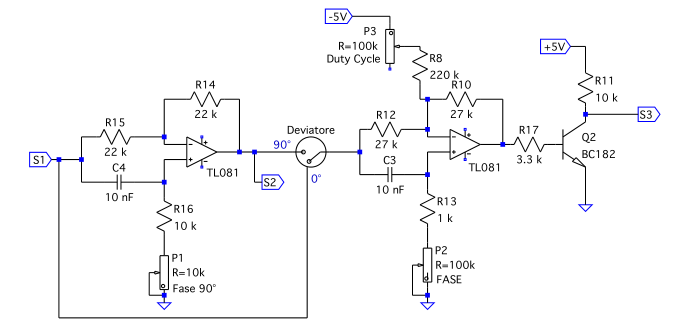
\includegraphics[scale=0.75]{sfasatori.png}
\caption{Schema circuitale dello sfasatore di 90\degree e dello sfasatore variabile.\label{fig:sfasatori}}
\end{figure}


\subparagraph{Squadratore e campionatore}
Abbiamo montato i circuiti in figura \ref{fig:sqadratore-campionatore}. Ricordiamo che S3 corrisponde all'onda quadra in uscita dallo sfasatore variabile e viene inviato ai due NOT U1 e U2 (che hanno la funzione di ripulire il segnale), quindi il segnale S4 e il suo negato S5 vengono mandati al campionatore realizzato con un circuito integrato contenente interruttori MOSFET. Seguendo la logica del circuito in figura si vede che S6 e S5 selezionano alternativamente l'uscita S8 o S7 su cui mandare il segnale S6. L'uscita che non lo riceve viene in quel semiperiodo messa a terra.\\

IMMAGINI DELLE ONDE
S4 e S5 IN OPPOSIZIONE DI FASE
S7 E S8 NELLE CONFIGURAZIONI DEL DEVIATORE

\begin{figure}[!htb]
  \centering
  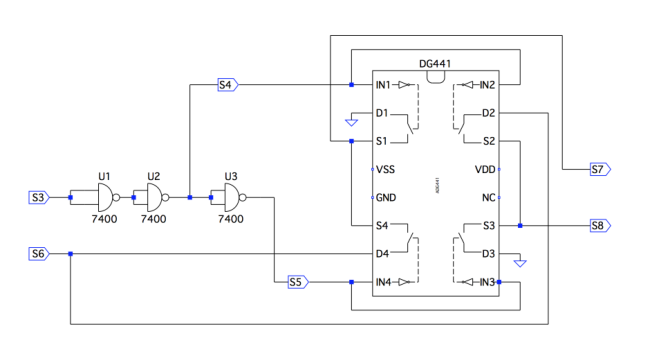
\includegraphics[scale=0.75]{sqadratore-campionatore.png}
\caption{Schema circuitale dello squadratore e del campionatore.\label{fig:sqadratore-campionatore}}
\end{figure}


\subparagraph{Amplificatore differenziale e mediatore}
Infine abbiamo realizzato il circuito in figura \ref{fig:amplificatorediff-mediatore}. Le onde agli ingressi S7 e S8 sono sommate dall'amplificatore differenziale, il quale amplifica in realtà la differenza, così da ottenere un output a segno definito. Infine due integratori (uno RC e l'altro con opAmp) rendono continuo il segnale. Le frequenze di taglio di entrambi sono dell'ordine delle decine di Hz, dunque per il segnale a $1$kHz funzionano bene come integratori.

IMMAGINI DI TUTTE LE ONDE CON DEVIATORE 0/90
ONDA S9 PER POSIZIONI DEVIATORE%ci si aspetta sempre stesso segno/segnale a media nulla
VOLTMETRO DEVE DARE MEDIA DEL SEGNALE IN INGRESSO (se sfaso di 90)
IMMAGINE TENSIONE CONTINUA
REGOLARE FASE P2 T.C. CON 90 VOLTMETRO=0 %compensazione fasi
NELLA POSIZIONE 0 vedio tensione diversa da 0

\begin{figure}[!htb]
  \centering
  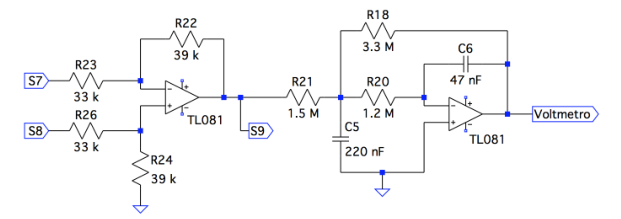
\includegraphics[scale=0.75]{amplificatorediff-mediatore.png}
\caption{Schema a blocchi del circuito Lock-in.\label{fig:amplificatorediff-mediatore}}
\end{figure}

\section{Presa dati}

TABELLA DATI
IMMAGINE E FIT




\section{Conclusioni}

CONFRONTO DEI VALORI OTTENUTI CON E SENZA LOCK-IN E COMMENTI


\begin{table}[!htb]
\centering
\begin{tabular}{|c|c|c|c|}
\hline 
$R_i [\Omega ]$ & $\Delta R_i [\Omega ]$ & $t [\mu s]$ & $\Delta t [\mu s]$\\
\hline
 327 &  3 & 25.8 & 0.2\\ 
\hline 
 470 &  4 & 41.6 & 0.2\\ 
\hline
 669 &  5 & 69.2 & 0.6\\ 
\hline
 824 &  7 & 82 & 1\\ 
\hline 
 984 &  8 & 102 & 1\\ 
\hline
 1183 &  9 & 118 & 1\\ 
\hline
 1454 &  11 & 140 & 1\\ 
\hline
\end{tabular} 
\caption{Presa dati per verificare la linearità fra $R$ e $t$.\label{tab:monostabile}}
\end{table}


\end{document}